\documentclass[aspectratio=169,9pt,xcolor=table]{beamer}

\usepackage[T1]{fontenc}
\usepackage{helvet}
\usepackage{amsmath}
\usepackage{booktabs}
\usepackage{graphicx}
\usepackage{tabularx}
\usepackage{tikz}
\usetikzlibrary{positioning}
\usepackage{hyperref}

\renewcommand{\familydefault}{\sfdefault}
\graphicspath{{cognitive_gaze_figures/}{./}}
\setbeamertemplate{navigation symbols}{}
\setbeamertemplate{itemize item}{\color{Teal}$\bullet$}
\setbeamertemplate{itemize subitem}{\color{Blue}$\circ$}

\definecolor{Navy}{HTML}{122B3E}
\definecolor{Teal}{HTML}{007D84}
\definecolor{Blue}{HTML}{316FAA}
\definecolor{Amber}{HTML}{BC7918}
\definecolor{Red}{HTML}{AD413D}
\definecolor{Ink}{HTML}{2B3034}
\definecolor{Mid}{HTML}{5E666C}
\definecolor{Light}{HTML}{D3D8DA}
\definecolor{OffWhite}{HTML}{F9F9F6}
\definecolor{PaleTeal}{HTML}{E2F2F1}
\definecolor{PaleBlue}{HTML}{E7EFF7}
\definecolor{PaleAmber}{HTML}{FBF1D9}
\definecolor{PaleRed}{HTML}{F5DEDC}
\definecolor{Purple}{HTML}{7A5AA6}

\setbeamercolor{normal text}{fg=Ink,bg=OffWhite}
\setbeamercolor{frametitle}{fg=Navy,bg=OffWhite}
\setbeamercolor{structure}{fg=Teal}
\setbeamerfont{frametitle}{size=\Large,series=\bfseries}
\setbeamertemplate{frametitle}{
  \vspace{0.22cm}
  \insertframetitle\par
  \vspace{0.08cm}
  {\color{Light}\rule{\textwidth}{0.5pt}}
}
\setbeamertemplate{footline}{
  \leavevmode
  \hbox{
    \begin{beamercolorbox}[wd=.90\paperwidth,ht=2.7ex,dp=1.2ex,leftskip=.45cm]{author in head/foot}
      \color{Mid}\scriptsize Kodiak Sciences --- cognitive gaze-tracking evidence deck
    \end{beamercolorbox}
    \begin{beamercolorbox}[wd=.10\paperwidth,ht=2.7ex,dp=1.2ex,center]{date in head/foot}
      \color{Navy}\scriptsize\insertframenumber
    \end{beamercolorbox}
  }
}

\newcommand{\evidence}[2]{%
  \vspace{-0.06cm}\hfill
  \colorbox{#2}{\color{white}\bfseries\scriptsize\strut\ #1\ }\par
  \vspace{0.04cm}
}
\newcommand{\source}[1]{\vfill{\color{Mid}\tiny Source: #1}}
\newcommand{\takeaway}[1]{%
  \begin{beamercolorbox}[rounded=true,sep=0.10cm,wd=\textwidth]{block body}
    \color{Navy}\bfseries #1
  \end{beamercolorbox}
}
\newcommand{\card}[3]{%
  \begin{beamercolorbox}[rounded=true,sep=0.12cm,wd=\linewidth]{#1}
    {\color{Navy}\bfseries #2}\par\vspace{0.04cm}{\small #3}
  \end{beamercolorbox}
}
\newcommand{\compactcard}[3]{%
  \begin{beamercolorbox}[rounded=true,sep=0.08cm,wd=\linewidth]{#1}
    {\color{Navy}\bfseries\scriptsize #2}\par{\scriptsize #3}
  \end{beamercolorbox}
}
\setbeamercolor{block body}{bg=PaleBlue,fg=Ink}
\setbeamercolor{tealcard}{bg=PaleTeal,fg=Ink}
\setbeamercolor{bluecard}{bg=PaleBlue,fg=Ink}
\setbeamercolor{ambercard}{bg=PaleAmber,fg=Ink}
\setbeamercolor{redcard}{bg=PaleRed,fg=Ink}

\title{How an SD-SLO Measures Eye Motion}
\subtitle{A first-principles guide from hardware and scan timing to cognitive-platform requirements}
\author{Kodiak Sciences gaze-tracking program}
\date{22 July 2026}

\begin{document}

\begin{frame}[plain]
  \begin{tikzpicture}[remember picture,overlay]
    \fill[Navy] (current page.south west) rectangle (current page.north east);
    \fill[Teal] (current page.south west) rectangle ([xshift=.18\paperwidth]current page.north west);
  \end{tikzpicture}
  \vspace{0.85cm}
  \hspace{1.35cm}
  \begin{minipage}{0.70\paperwidth}
    {\color{white}\fontsize{26}{29}\selectfont\bfseries
      How an SD-SLO\\measures eye motion\par}
    \vspace{0.5cm}
    {\color{PaleTeal}\Large
      A first-principles guide for readers who do not already know the instrument,
      its timing model, or the gaze-estimation pipeline\par}
    \vspace{1.0cm}
    {\color{white}\small Status: 2026-07-22 \quad$\bullet$\quad
      numerical claims are evidence-classified}
  \end{minipage}
\end{frame}

\begin{frame}{What this document will explain}
  \evidence{READING MAP}{Navy}
  \begin{columns}[T,onlytextwidth]
    \column{0.48\textwidth}
      \begin{enumerate}
        \item What an SLO is and how its optical/electronic components create a raster
        \item Why a retinal image contains time, not only space
        \item How strips and normalized correlation estimate motion
        \item How pixel displacement becomes a calibrated gaze trajectory
      \end{enumerate}
    \column{0.48\textwidth}
      \begin{enumerate}\setcounter{enumi}{4}
        \item What current synthetic and real-data results do and do not prove
        \item Why inter-frame dead time matters for cognitive events
        \item Which signals need temporal rate versus spatial precision
        \item Which production interfaces should be frozen before hardware
      \end{enumerate}
  \end{columns}
  \vspace{0.35cm}
  \begin{beamercolorbox}[rounded=true,sep=.14cm]{bluecard}
    \textbf{How to read the evidence labels.} ``Measured'' means observed on a stated capture;
    ``derived'' means arithmetic from stated inputs; ``fixture'' means synthetic known truth;
    ``hypothesis'' and ``missing'' explicitly mark claims that still require measurement.
  \end{beamercolorbox}
  \source{scope of this explanatory deck}
\end{frame}

\begin{frame}{An SLO is a point-scanning camera for the retina}
  \evidence{HARDWARE PRIMER}{Navy}
  \begin{columns}[T,onlytextwidth]
    \column{0.49\textwidth}
      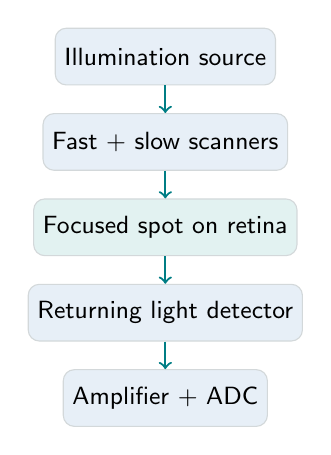
\begin{tikzpicture}[
        box/.style={draw=Light,rounded corners,minimum width=2.3cm,minimum height=.72cm,
                    align=center,fill=PaleBlue,font=\small},
        arr/.style={->,thick,Teal}
      ]
        \node[box] (laser) {Illumination source};
        \node[box,below=.35cm of laser] (scanner) {Fast + slow scanners};
        \node[box,below=.35cm of scanner,fill=PaleTeal] (eye) {Focused spot on retina};
        \node[box,below=.35cm of eye] (detector) {Returning light detector};
        \node[box,below=.35cm of detector] (adc) {Amplifier + ADC};
        \draw[arr] (laser)--(scanner); \draw[arr] (scanner)--(eye);
        \draw[arr] (eye)--(detector); \draw[arr] (detector)--(adc);
      \end{tikzpicture}
    \column{0.47\textwidth}
      \textbf{Scanning laser ophthalmoscope (SLO).}
      A small optical spot is moved across the retina. The detector records one intensity
      value at each instant. Scanner position and detector time together determine where that
      sample belongs in the retinal image.

      \vspace{0.25cm}
      \textbf{Why this matters for gaze.}
      If the eye moves while the raster is being acquired, vessels shift between early and late
      samples. Registration estimates that shift. The gaze signal is therefore derived from the
      time-dependent deformation of retinal structure, not from a separate pupil image.
  \end{columns}
  \source{instrument-level interpretation of the technical note and repository scan model}
\end{frame}

\begin{frame}{Two scanner axes create one image}
  \evidence{HARDWARE PRIMER + DERIVED}{Blue}
  \begin{columns}[T,onlytextwidth]
    \column{0.49\textwidth}
      \card{tealcard}{FAST AXIS}{
        The resonant scanner sweeps the spot horizontally. At 10 kHz, one full sinusoid lasts
        100 $\mu$s. Using both half-cycles yields a forward line and a reverse line, each 50 $\mu$s.}
      \vspace{0.2cm}
      \card{bluecard}{SLOW AXIS}{
        A second scanner advances the beam vertically from line to line. A nominal frame is the
        software grouping of many sequential fast-axis lines.}
    \column{0.47\textwidth}
      \begin{align*}
        T_{\mathrm{sine}} &= 1/f_{\mathrm{scan}} = 100~\mu\mathrm{s}\\
        T_{\mathrm{line}} &= T_{\mathrm{sine}}/2 = 50~\mu\mathrm{s}\\
        f_{\mathrm{line}} &= 2f_{\mathrm{scan}} = 20{,}000~\mathrm{s}^{-1}\\
        T_{808} &= 808/f_{\mathrm{line}} = 40.4~\mathrm{ms}
      \end{align*}
      These numbers describe the candidate 10 kHz fast axis. They do not by themselves reveal
      slow-axis return time, optical blanking, or the duty cycle of the current capture.
  \end{columns}
  \source{technical note sections 1--3; legacy 808-line geometry}
\end{frame}

\begin{frame}{The detector produces a time series before it produces an image}
  \evidence{FIRST PRINCIPLES}{Blue}
  \begin{columns}[T,onlytextwidth]
    \column{0.50\textwidth}
      Let detector samples be $I(t_k)$ and scanner position be $(x(t_k),y(t_k))$.
      Image formation assigns each sample to a retinal coordinate:
      \[
        \{I(t_k),x(t_k),y(t_k)\}_{k=1}^{N}
        \longrightarrow I_{\mathrm{rect}}(x_i,y_j).
      \]
      The raw ADC is uniform in time. Because a sinusoid moves fastest at field center and stops
      at the turnarounds, those samples are \emph{not} uniform in retinal space.
    \column{0.46\textwidth}
      \card{bluecard}{A FRAME IS A CONVENTION}{
        A frame is a block of sequential lines chosen for image construction. The retina was not
        measured everywhere at one instant.}
      \vspace{0.2cm}
      \card{redcard}{A MISSING INTERVAL IS PHYSICAL}{
        If lines are not recorded during slow-axis return or blanking, no image-processing method
        can recreate the unobserved retinal photons.}
  \end{columns}
  \source{technical note sampling model; scan\_timing.py; desinusoid.py}
\end{frame}

\begin{frame}{Eye motion is written into the raster as distortion}
  \evidence{FIRST PRINCIPLES}{Blue}
  \begin{columns}[T,onlytextwidth]
    \column{0.51\textwidth}
      Suppose a vessel has stationary retinal texture $R(x,y)$ and the eye displacement is
      $\mathbf d(t)=[d_x(t),d_y(t)]^\mathsf{T}$. The detector approximately sees
      \[
        I(t)\approx R\!\left(x_s(t)-d_x(t),\,y_s(t)-d_y(t)\right)+\eta(t),
      \]
      where $(x_s,y_s)$ is scanner position and $\eta$ is detector/texture noise.
      Different parts of one frame therefore encode different eye positions.
    \column{0.45\textwidth}
      \textbf{Registration inverts this effect.}
      A short strip spans a small time aperture. Matching that strip to a retinal reference estimates
      the displacement that best aligns the vessel pattern.

      \vspace{0.25cm}
      \textbf{Trade-off.}
      Wider strips contain more vessel structure and improve correlation, but average motion over a
      longer interval. Smaller stride emits estimates more often, but neighboring estimates reuse pixels.
  \end{columns}
  \source{brightness-constancy motion model; strip registration implementation}
\end{frame}

\begin{frame}{The mission changed; the architecture mostly did not}
  \evidence{PROGRAM FACT + ARCHITECTURE}{Navy}
  \begin{columns}[T,onlytextwidth]
    \column{0.47\textwidth}
      \card{bluecard}{2020 vector: home retinal health}{
        \begin{itemize}
          \item Portable SLO/OCT imaging
          \item Intermittent, high-quality retinal frames
          \item Patient monitoring between clinic visits
          \item Image quality and medical workflow dominate
        \end{itemize}}
    \column{0.47\textwidth}
      \card{tealcard}{Current vector: cognitive platform}{
        \begin{itemize}
          \item Continuous attention-aligned measurements
          \item Retina, pupil, stimulus, behavior, and OPM-MEG
          \item Hardware time, validity, uncertainty, and provenance
          \item Model-ready synchronized sequences
        \end{itemize}}
  \end{columns}
  \vspace{0.25cm}
  \takeaway{Keep the retinal capability; re-audit assumptions that let frame boundaries erase time.}
  \source{program history; OPM coexistence accepted as characterized}
\end{frame}

\begin{frame}{Every number carries an evidence class}
  \evidence{EVIDENCE POLICY}{Navy}
  \begin{columns}[T,onlytextwidth]
    \column{0.32\textwidth}
      \card{tealcard}{MEASURED}{Directly measured on the stated capture or hardware.}
      \vspace{0.12cm}
      \card{bluecard}{DERIVED}{Calculated from cited inputs with an explicit formula.}
      \vspace{0.12cm}
      \card{bluecard}{LITERATURE}{Reported by a primary or authoritative source.}
    \column{0.32\textwidth}
      \card{ambercard}{FIXTURE}{Known-truth software or synthetic experiment.}
      \vspace{0.12cm}
      \card{bluecard}{PROGRAM FACT}{Accepted project history or characterized capability.}
      \vspace{0.12cm}
      \card{redcard}{HYPOTHESIS}{Candidate design or interpretation requiring validation.}
    \column{0.32\textwidth}
      \card{redcard}{MISSING}{Required value absent; no numerical conclusion is permitted.}
      \vspace{0.25cm}
      \begin{itemize}
        \item No synthetic-to-biological upgrade
        \item No prediction-to-observation upgrade
        \item No geometry-to-safety upgrade
      \end{itemize}
  \end{columns}
  \source{cognitive\_gaze\_evidence.json}
\end{frame}

\begin{frame}{From photons to an attention-aligned sample}
  \evidence{SYSTEM PIPELINE}{Navy}
  \begin{center}
  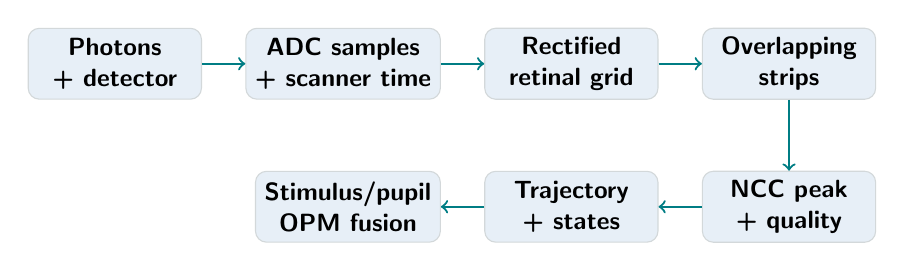
\begin{tikzpicture}[
    node distance=0.55cm,
    box/.style={draw=Light,rounded corners,minimum width=2.2cm,minimum height=0.9cm,
                align=center,fill=PaleBlue,font=\small\bfseries},
    arrow/.style={->,thick,Teal}
  ]
    \node[box] (p) {Photons\\+ detector};
    \node[box,right=of p] (a) {ADC samples\\+ scanner time};
    \node[box,right=of a] (r) {Rectified\\retinal grid};
    \node[box,right=of r] (s) {Overlapping\\strips};
    \node[box,below=0.9cm of s] (n) {NCC peak\\+ quality};
    \node[box,left=of n] (t) {Trajectory\\+ states};
    \node[box,left=of t] (f) {Stimulus/pupil\\OPM fusion};
    \draw[arrow] (p)--(a); \draw[arrow] (a)--(r); \draw[arrow] (r)--(s);
    \draw[arrow] (s)--(n); \draw[arrow] (n)--(t); \draw[arrow] (t)--(f);
  \end{tikzpicture}
  \end{center}
  \vspace{0.35cm}
  \takeaway{Invariant record: acquisition time, direction, calibration version, quality,
    and observed/predicted/rejected/missing state.}
  \source{technical note; repository contracts; architecture synthesis}
\end{frame}

\begin{frame}{``Rate'' is four different clocks}
  \evidence{DERIVED}{Blue}
  \begin{columns}[T,onlytextwidth]
    \column{0.24\textwidth}
      \card{tealcard}{LINE CLOCK}{20 kline/s\\One 50 $\mu$s half-sine per line}
    \column{0.24\textwidth}
      \card{bluecard}{APERTURE CLOCK}{1.20 ms\\24 lines contribute to one estimate}
    \column{0.24\textwidth}
      \card{ambercard}{UPDATE CLOCK}{0.30 ms\\6-line stride gives 3.33 kHz spacing}
    \column{0.24\textwidth}
      \card{redcard}{WALL CLOCK}{Duty limited\\Active updates stop in dead time}
  \end{columns}
  \vspace{0.45cm}
  \takeaway{Overlapping estimates are correlated. Output spacing is not independent measurement bandwidth.}
  \source{technical note; 24/6 strip design example}
\end{frame}

\begin{frame}{A 10 kHz sine is a 20 kline/s bidirectional clock}
  \evidence{DERIVED}{Blue}
  \centering
  \includegraphics[width=0.93\textwidth,height=0.73\textheight,keepaspectratio]{01_scan_physics.png}
  \source{technical note sections 2--3 and 7}
\end{frame}

\begin{frame}{Angular field becomes millimeters through the eye model}
  \evidence{HYPOTHESIS + DERIVED}{Red}
  \begin{columns}[T,onlytextwidth]
    \column{0.48\textwidth}
      \begin{align*}
        q &= 0.01306(AL-1.82)\\
        q(24~\mathrm{mm}) &= 0.2896708~\mathrm{mm/deg}\\
        W &= 48^\circ q = 13.9042~\mathrm{mm}
      \end{align*}
    \column{0.48\textwidth}
      \card{redcard}{Model boundary}{
        The 24 mm axial length and 48$^\circ$ field are nominal design inputs.
        Subject-specific millimeters require measured biometry and calibrated scan geometry.}
  \end{columns}
  \vspace{0.35cm}
  \takeaway{Pixel displacement is measured first; retinal angle or millimeters require explicit calibration.}
  \source{technical note sections 1--2; Bennett et al. 1994}
\end{frame}

\begin{frame}{Bandwidth, optics, and stored pixels are not interchangeable}
  \evidence{MEASURED + DERIVED + HYPOTHESIS}{Blue}
  \centering
  \includegraphics[width=0.94\textwidth,height=0.73\textheight,keepaspectratio]{02_resolution_sampling.png}
  \source{technical note sections 4--8}
\end{frame}

\begin{frame}{Desinusoiding changes coordinates---not information}
  \evidence{METHOD INVARIANT}{Navy}
  \begin{columns}[T,onlytextwidth]
    \column{0.48\textwidth}
      \begin{align*}
        x(t) &= A\sin(2\pi f t + \phi)\\
        I(t) &\longrightarrow I\!\left(t(x)\right)
      \end{align*}
      \begin{itemize}
        \item Apply measured position LUT when available
        \item Correct detector/scanner delay before interpolation
        \item Preserve direction and invalid turnaround states
      \end{itemize}
    \column{0.48\textwidth}
      \card{redcard}{What rectification cannot do}{
        It cannot recover analog bandwidth, photons, or samples that were never acquired.
        It only maps time-ordered data onto a declared retinal coordinate.}
  \end{columns}
  \source{desinusoid.py; scan model; technical note}
\end{frame}

\begin{frame}{The image is a time-ordered measurement---not a snapshot}
  \evidence{FIRST PRINCIPLES}{Blue}
  \begin{columns}[T,onlytextwidth]
    \column{0.54\textwidth}
      \includegraphics[width=\linewidth,height=0.60\textheight,keepaspectratio]{snr_diagnostic.png}
    \column{0.42\textwidth}
      \card{tealcard}{Raster interpretation}{
        Each stored column/line corresponds to a different acquisition time.
        Eye motion therefore appears as retinal shear and displacement within a nominal frame.}
      \vspace{0.2cm}
      \card{bluecard}{Required metadata}{
        Line start, sample period, direction, position calibration, validity reason,
        optical state, and hardware clock.}
  \end{columns}
  \source{test1 real retinal capture; measured SNR diagnostic}
\end{frame}

\begin{frame}{Strip width sets aperture; stride sets output spacing}
  \evidence{DERIVED + FIXTURE}{Amber}
  \centering
  \includegraphics[width=0.94\textwidth,height=0.73\textheight,keepaspectratio]{04_strip_overlap.png}
  \source{20 kline/s candidate clock; 24-line width; 6-line stride}
\end{frame}

\begin{frame}{Width and stride control different physical quantities}
  \evidence{DERIVED EXAMPLE}{Blue}
  \begin{columns}[T,onlytextwidth]
    \column{0.49\textwidth}
      For strip width $W$, stride $S$, and line rate $f_L$:
      \begin{align*}
        T_{\mathrm{aperture}} &= W/f_L,\\
        T_{\mathrm{spacing}} &= S/f_L,\\
        f_{\mathrm{output}} &= f_L/S,\\
        \mathrm{shared\ fraction} &= 1-S/W.
      \end{align*}
      With $W=24$, $S=6$, and $f_L=20{,}000$ lines/s:
      \[
        T_{\mathrm{aperture}}=1.20~\mathrm{ms},\quad
        T_{\mathrm{spacing}}=0.30~\mathrm{ms}.
      \]
    \column{0.47\textwidth}
      \textbf{Interpretation.}
      Each estimate integrates retinal structure over 1.20 ms, yet an estimate is emitted every
      0.30 ms. Consecutive estimates share 18 of 24 lines (75\%).

      \vspace{0.25cm}
      \textbf{Consequence.}
      The 3.33 kHz output sequence is useful for localizing changes in time, but it is not 3.33 kHz
      of independent photon evidence. Aperture blur, overlap, detector bandwidth, and registration
      noise still limit recoverable motion.
  \end{columns}
  \source{technical note candidate line clock; strip-design example in evidence ledger}
\end{frame}

\begin{frame}{The registration loop, end to end}
  \evidence{IMPLEMENTED METHOD}{Navy}
  \centering
  \includegraphics[width=0.94\textwidth,height=0.73\textheight,keepaspectratio]{03_pipeline_walkthrough.png}
  \source{intraframe\_ncc preprocessing, reference, registration, and trajectory modules}
\end{frame}

\begin{frame}{Normalized correlation asks for shape, not brightness}
  \evidence{METHOD}{Navy}
  \begin{columns}[T,onlytextwidth]
    \column{0.54\textwidth}
      \[
      \resizebox{0.98\linewidth}{!}{$
        \operatorname{NCC}(u,v)=
        \frac{\sum_{x,y}[T(x,y)-\bar T][R(x+u,y+v)-\bar R_{u,v}]}
        {\sqrt{\sum_{x,y}[T(x,y)-\bar T]^2
               \sum_{x,y}[R(x+u,y+v)-\bar R_{u,v}]^2}}
      $}
      \]
      \begin{itemize}
        \item Local means remove broad brightness offsets
        \item Normalized energy bounds similarity
        \item A bounded search region constrains displacement
      \end{itemize}
    \column{0.42\textwidth}
      \card{tealcard}{Preprocessing}{Debanding/local-mean removal and DoG filtering expose
        vessel edges without increasing biological resolution.}
      \vspace{0.2cm}
      \card{redcard}{Quality boundary}{Low, ambiguous, or boundary-saturated peaks remain rejected.}
  \end{columns}
  \source{OpenCV TM\_CCOEFF\_NORMED; register.py}
\end{frame}

\begin{frame}{How to read a correlation surface}
  \evidence{METHOD EXPLANATION}{Navy}
  \begin{columns}[T,onlytextwidth]
    \column{0.50\textwidth}
      The algorithm shifts the moving strip over a bounded reference search region. At each
      candidate displacement $(u,v)$ it computes one NCC value. The result is a 2-D surface:
      \begin{itemize}
        \item peak location $\rightarrow$ best displacement;
        \item peak height $\rightarrow$ similarity/quality;
        \item peak shape $\rightarrow$ ambiguity and local curvature;
        \item boundary peak $\rightarrow$ requested motion may exceed the search region.
      \end{itemize}
    \column{0.46\textwidth}
      \textbf{Subpixel refinement.}
      Integer-pixel matching is refined independently in $x$ and $y$ using a three-point
      parabolic vertex around the discrete maximum. This estimates the local maximum of the
      sampled response; it does not create new optical resolution.

      \vspace{0.25cm}
      \textbf{Acceptance.}
      A sample is OBSERVED only when acquisition is valid and registration quality passes.
      Otherwise it is REJECTED or MISSING; prediction is a separate downstream state.
  \end{columns}
  \source{register.py; trajectory.py; production state contract}
\end{frame}

\begin{frame}{A correlation peak becomes a placed vessel pattern}
  \evidence{IMPLEMENTED + VISUALIZED}{Navy}
  \centering
  \includegraphics[width=0.92\textwidth,height=0.72\textheight,keepaspectratio]{05_ncc_placement.png}
  \source{integer peak shown for clarity; production uses three-point parabolic refinement}
\end{frame}

\begin{frame}{Repeat the placement across scan time to recover a trajectory}
  \evidence{MEASURED, UNSCORED}{Teal}
  \begin{columns}[T,onlytextwidth]
    \column{0.58\textwidth}
      \includegraphics[width=\linewidth,height=0.64\textheight,keepaspectratio]{real_demo.png}
    \column{0.38\textwidth}
      \begin{enumerate}
        \item Strip center defines acquisition time
        \item NCC peak defines displacement
        \item Quality defines accepted or rejected
        \item States remain explicit in output
      \end{enumerate}
      \vspace{0.2cm}
      \card{redcard}{Claim boundary}{45/47 strips lock in this frame; there is no independent
        high-rate biological truth.}
  \end{columns}
  \source{test1 frame 875; intraframe real demonstration}
\end{frame}

\begin{frame}{A trajectory sample has a value, a time, and provenance}
  \evidence{DATA CONTRACT}{Navy}
  A useful gaze row is more than $(x,y)$. It should include:
  \[
    z_i =
    \left[
      t_i,\ \Delta x_i,\ \Delta y_i,\ q_i,
      a_i,\ e_i,\ p_i,\ c_i,\ r_i
    \right],
  \]
  where $q_i$ is registration quality, $a_i$ acquisition state, $e_i$ estimate state,
  $p_i$ prediction provenance, $c_i$ calibration version, and $r_i$ hardware/software revision.

  \vspace{0.25cm}
  \begin{columns}[T,onlytextwidth]
    \column{0.48\textwidth}
      \textbf{Why the time is the strip center.}
      The strip integrates several lines; assigning the estimate to the aperture center makes its
      timing explicit and avoids pretending the displacement was instantaneous.
    \column{0.48\textwidth}
      \textbf{Why provenance remains attached.}
      Calibration, scanner geometry, optical mode, and estimator settings determine how pixels
      become physical gaze. Removing them makes later multimodal alignment and validation ambiguous.
  \end{columns}
  \source{contracts.py; trajectory.py; proposed line-record interface}
\end{frame}

\begin{frame}{Pixels become gaze only through explicit calibration}
  \evidence{CALIBRATION REQUIREMENT}{Navy}
  \begin{columns}[T,onlytextwidth]
    \column{0.48\textwidth}
      \begin{align*}
        \Delta\theta_x &= s_x\,\Delta x_{\mathrm{px}}\\
        \Delta\theta_y &= s_y\,\Delta y_{\mathrm{px}}
      \end{align*}
      \begin{itemize}
        \item Image axes and scanner axes
        \item Sign and handedness
        \item Retinal angle and display coordinates
        \item Calibration source and version
      \end{itemize}
    \column{0.48\textwidth}
      \card{redcard}{Fail loudly}{
        Missing calibration leaves positions in pixels.
        The pipeline must not invent arcminutes or millimeters.}
      \vspace{0.2cm}
      \card{bluecard}{Separate problem}{
        Axial-length scaling converts angle to retinal distance;
        it is not part of image registration.}
  \end{columns}
  \source{contracts.py; calibration configuration; technical note eye model}
\end{frame}

\begin{frame}{The reference image is part of the measurement model}
  \evidence{METHOD + LIMITATION}{Navy}
  \begin{columns}[T,onlytextwidth]
    \column{0.31\textwidth}
      \card{bluecard}{INCREMENTAL}{High overlap; relative trajectory; accumulated drift.}
    \column{0.31\textwidth}
      \card{tealcard}{FIXED / ATLAS}{Absolute reference; vulnerable to field-of-view exit.}
    \column{0.31\textwidth}
      \card{ambercard}{SELF-CONSISTENT}{Improves lock coverage; can absorb shared motion.}
  \end{columns}
  \vspace{0.4cm}
  \takeaway{A same-acquisition atlas is useful registration structure, but it is not independent gaze truth.}
  \source{reference.py; self-consistent median reference implementation}
\end{frame}

\begin{frame}{Credibility is a ladder; each rung answers a different question}
  \evidence{VALIDATION FRAMEWORK}{Navy}
  \begin{center}
  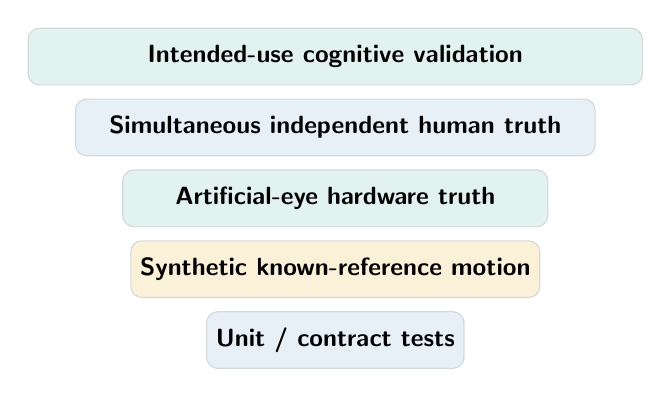
\begin{tikzpicture}[
    stepbox/.style={draw=Light,rounded corners,minimum height=.72cm,align=center,font=\small\bfseries}
  ]
    \node[stepbox,fill=PaleBlue,minimum width=3.0cm] at (0,0) {Unit / contract tests};
    \node[stepbox,fill=PaleAmber,minimum width=4.2cm] at (0,0.9) {Synthetic known-reference motion};
    \node[stepbox,fill=PaleTeal,minimum width=5.4cm] at (0,1.8) {Artificial-eye hardware truth};
    \node[stepbox,fill=PaleBlue,minimum width=6.6cm] at (0,2.7) {Simultaneous independent human truth};
    \node[stepbox,fill=PaleTeal,minimum width=7.8cm] at (0,3.6) {Intended-use cognitive validation};
  \end{tikzpicture}
  \end{center}
  \takeaway{Synthetic precision validates the estimator under its model; it does not establish biological waveform accuracy.}
  \source{repository tests, synthetic fixtures, and proposed validation program}
\end{frame}

\begin{frame}{Measured image statistics set the synthetic operating regime}
  \evidence{MEASURED SNR + FIXTURE}{Amber}
  \begin{columns}[T,onlytextwidth]
    \column{0.62\textwidth}
      \includegraphics[width=\linewidth,height=0.65\textheight,keepaspectratio]{operating_curve.png}
    \column{0.34\textwidth}
      \card{tealcard}{Measured input}{Median structure SNR: 15.242 dB\\
        bootstrap interval: 14.485--15.886 dB}
      \vspace{0.18cm}
      \card{ambercard}{Known-truth point}{24/6, DoG(1,8), spatial NCC:\\
        0.05221 arcmin RMSE; 393/393 locks}
      \vspace{0.18cm}
      \card{redcard}{Boundary}{Precision is valid only under the declared synthetic model.}
  \end{columns}
  \source{snr.json; operating\_curve.json; FINDINGS.md}
\end{frame}

\begin{frame}{A 10 ms synthetic waveform is recoverable under the stated model}
  \evidence{FIXTURE}{Amber}
  \begin{columns}[T,onlytextwidth]
    \column{0.63\textwidth}
      \centering
      \includegraphics[width=0.88\linewidth,height=0.56\textheight,keepaspectratio]{waveform_recovery.png}
    \column{0.33\textwidth}
      \compactcard{ambercard}{Fixture}{10 arcmin / 10 ms vertical (fast/image-row) event; real-frame-derived
        morphology; 15\% speckle + Gaussian noise; 32/4 operating point.}
      \vspace{0.18cm}
      \compactcard{tealcard}{Observed in fixture}{3/3 recovered at both 40.0 and 58.3 ms active-time brackets.}
      \vspace{0.18cm}
      \compactcard{redcard}{Uncertainty}{The 3/3 Wilson interval is 0.439--1.000; recovery probability remains uncertain.}
  \end{columns}
  \source{waveform\_recovery.json}
\end{frame}

\begin{frame}{Real retinal data demonstrate lock behavior---not truth}
  \evidence{MEASURED, UNSCORED}{Teal}
  \begin{columns}[T,onlytextwidth]
    \column{0.62\textwidth}
      \includegraphics[width=\linewidth,height=0.66\textheight,keepaspectratio]{real_demo.png}
    \column{0.34\textwidth}
      \begin{itemize}
        \item Frame 875
        \item 45/47 strips locked
        \item Median locked NCC 0.6246
        \item Structured residual and plausible shear
      \end{itemize}
      \card{redcard}{Not established}{No independent high-rate eye-motion truth; displacement
        and waveform accuracy cannot be scored.}
  \end{columns}
  \source{real\_demo.json; test1 capture}
\end{frame}

\begin{frame}{The legacy pipeline tracks held-out pursuit at a coarse level}
  \evidence{MEASURED + ASSUMED TIMING}{Teal}
  \centering
  \includegraphics[width=0.93\textwidth,height=0.72\textheight,keepaspectratio]{08_pursuit_result.png}
  \source{champion pursuit result; fixture's unmeasured 10 ms dead-time hypothesis}
\end{frame}

\begin{frame}{What the current evidence supports}
  \evidence{CLAIM BOUNDARY}{Navy}
  \begin{columns}[T,onlytextwidth]
    \column{0.48\textwidth}
      \card{tealcard}{SUPPORTED NOW}{
        \begin{itemize}
          \item Real retinal structure supports strip locking
          \item Synthetic known-truth registration is precise
          \item Synthetic 10 ms waveform recovery is demonstrated
          \item Coarse pursuit correspondence is measured
          \item OPM coexistence is accepted as characterized
        \end{itemize}}
    \column{0.48\textwidth}
      \card{redcard}{NOT YET SUPPORTED}{
        \begin{itemize}
          \item Validated human microsaccade waveforms
          \item Hardware timing inferred from video alone
          \item Observations inside uncharacterized dead time
          \item Universal real-capture angular calibration
          \item Continuous-laser retinal safety determination
        \end{itemize}}
  \end{columns}
  \source{evidence ledger synthesis}
\end{frame}

\begin{frame}{The legacy frame boundary may create a cognitive blind interval}
  \evidence{CONDITIONAL DERIVATION}{Red}
  \centering
  \includegraphics[width=0.94\textwidth,height=0.72\textheight,keepaspectratio]{06_flyback_gap.png}
  \source{20 kline/s candidate clock; test1 808 lines and 14.633 fps}
\end{frame}

\begin{frame}{A good predictor cannot create an observation}
  \evidence{METHOD INVARIANT}{Navy}
  \begin{columns}[T,onlytextwidth]
    \column{0.24\textwidth}
      \card{tealcard}{OBSERVED}{Retinal photons acquired; quality gate passed.}
    \column{0.24\textwidth}
      \card{ambercard}{PREDICTED}{Dynamics model only; uncertainty expands.}
    \column{0.24\textwidth}
      \card{redcard}{REJECTED}{Photons acquired; registration not trusted.}
    \column{0.24\textwidth}
      \card{bluecard}{MISSING}{No usable acquisition; no measurement emitted.}
  \end{columns}
  \vspace{0.5cm}
  \takeaway{Cognitive event claims require observed photons across the event---or an explicit partial-observation claim.}
  \source{gap\_model.py; contracts.py measurement states}
\end{frame}

\begin{frame}{Continuous cognition does not require one fixed image format}
  \evidence{CANDIDATE ARCHITECTURE}{Red}
  \begin{columns}[T,onlytextwidth]
    \column{0.32\textwidth}
      \card{tealcard}{SCANNER A}{Bidirectional raster; best direct SLO continuity.}
    \column{0.32\textwidth}
      \card{bluecard}{SCANNER B}{Duty-optimized sawtooth; explicit residual turnaround.}
    \column{0.32\textwidth}
      \card{ambercard}{FUSION OVERLAY}{SLO precision plus eye-camera continuity; pairs with A or B.}
  \end{columns}
  \vspace{0.35cm}
  {\small\bfseries Freeze a versioned line record:}
  {\small sequence; clock/time/uncertainty; sample period; direction; position calibration;
  acquisition state; estimate state; prediction provenance; mode/revisions; optical/power state; intensity.}
  \vspace{0.25cm}
  \takeaway{Freeze scanner topology only after measured continuity, exposure, and image-quality tests.}
  \source{architecture candidates derived from production requirements}
\end{frame}

\begin{frame}{Choose sensors on two axes: time and space}
  \evidence{LITERATURE SYNTHESIS}{Purple}
  \centering
  \includegraphics[width=0.92\textwidth,height=0.72\textheight,keepaspectratio]{07_signal_landscape.png}
  \source{literature ranges and acquisition hypotheses in the evidence ledger}
\end{frame}

\begin{frame}{Different cognitive signals belong to different sensors}
  \evidence{LITERATURE SYNTHESIS}{Purple}
  \scriptsize
  \renewcommand{\arraystretch}{1.32}
  \begin{tabularx}{\textwidth}{>{\bfseries}l l l l X}
    \toprule
    Signal & Scale & Acquisition design & Precision & Primary sensor\\
    \midrule
    Saccade & $>1$--$2^\circ$ & 100--500; $\sim$1000 fine onset & arcmin & camera / SLO\\
    Micro onset/rate & $\sim0.1$--$0.5^\circ$ & $\geq250$; 500--1000 shape & coarse event & event camera / SLO\\
    Micro direction & endpoint vector & same event samples & sub-arcmin & SLO / fused\\
    Drift & to $\sim50$--$94'$\,s$^{-1}$ & 200--500 Hz & 0.5--1$'$; arcsec increments & SLO\\
    Tremor & often arcsec & $\geq500$ Hz practical & arcsec class & SLO / specialized\\
    Pupil & 2--8 mm & 20 content; 50--120 & 0.02--0.05 mm & eye camera\\
    \bottomrule
  \end{tabularx}
  \vspace{0.24cm}
  \begin{beamercolorbox}[rounded=true,sep=.14cm]{ambercard}
    \scriptsize Rates are acquisition targets, not event rates. Tremor has 40--100 Hz content:
    200 Hz is only the ideal floor and $\geq500$ Hz is practical.
    Arcsecond SD-SLO performance remains a validation target.
  \end{beamercolorbox}
  \source{Rucci \& Poletti 2015; Bowers et al. 2019; Rolfs 2009; Kelbsch et al. 2019}
\end{frame}

\begin{frame}{The cognitive product is a synchronized sensor graph}
  \evidence{PROGRAM FACT + ARCHITECTURE}{Navy}
  \begin{center}
  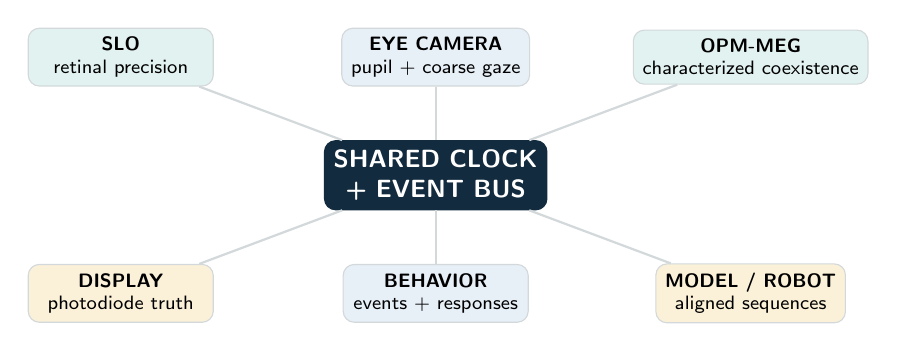
\begin{tikzpicture}[
    sensor/.style={draw=Light,rounded corners,minimum width=2.35cm,minimum height=.68cm,
                   align=center,fill=PaleBlue,font=\scriptsize},
    bus/.style={draw=Navy,rounded corners,minimum width=2.8cm,minimum height=.78cm,
                align=center,fill=Navy,text=white,font=\small\bfseries},
    link/.style={thick,Light}
  ]
    \node[bus] (bus) at (0,0) {SHARED CLOCK\\+ EVENT BUS};
    \node[sensor,fill=PaleTeal] (slo) at (-4,1.5) {\bfseries SLO\\retinal precision};
    \node[sensor] (cam) at (0,1.5) {\bfseries EYE CAMERA\\pupil + coarse gaze};
    \node[sensor,fill=PaleTeal] (opm) at (4,1.5) {\bfseries OPM-MEG\\characterized coexistence};
    \node[sensor,fill=PaleAmber] (display) at (-4,-1.5) {\bfseries DISPLAY\\photodiode truth};
    \node[sensor] (behavior) at (0,-1.5) {\bfseries BEHAVIOR\\events + responses};
    \node[sensor,fill=PaleAmber] (model) at (4,-1.5) {\bfseries MODEL / ROBOT\\aligned sequences};
    \foreach \x in {slo,cam,opm,display,behavior,model} \draw[link] (\x)--(bus);
  \end{tikzpicture}
  \end{center}
  \takeaway{OPM coexistence is accepted; production applicability remains bound to a controlled record and revision matrix.}
  \source{program architecture synthesis}
\end{frame}

\begin{frame}{``Laser safety'' is three separate regulatory questions}
  \evidence{SAFETY PRIMER}{Navy}
  \begin{columns}[T,onlytextwidth]
    \column{0.31\textwidth}
      \card{bluecard}{1. LASER PRODUCT CLASSIFICATION}{
        IEC 60825-1 and applicable 21 CFR provisions classify accessible emission and require
        product controls, including scanning safeguards.}
    \column{0.31\textwidth}
      \card{tealcard}{2. PATIENT EXPOSURE}{
        ISO 15004-2 or FDA-recognized ANSI Z80.36 evaluate ophthalmic-instrument exposure to the
        patient's eye under normal and fault conditions.}
    \column{0.31\textwidth}
      \card{ambercard}{3. MEDICAL DEVICE PATHWAY}{
        FDA device classification (for example product code MYC) governs regulatory pathway and
        recognized standards. It is not the same as IEC laser class.}
  \end{columns}
  \vspace{0.35cm}
  \textbf{Why scan geometry is insufficient.}
  A 10 kHz scan and nominal spot size describe where and how fast light moves. Exposure also
  depends on measured spectrum, power at the eye, beam profile, pupil coupling, complete two-axis
  trajectory and blanking, session duration, repeated visits, tolerances, and scanner-failure behavior.
  \source{IEC 60825-1; ISO 15004-2:2024; ANSI Z80.36-2021; FDA MYC and Laser Notice 56}
\end{frame}

\begin{frame}{Continuous scanning requires an exposure calculation---not a duty-cycle slogan}
  \evidence{PARAMETERIZED ONLY}{Mid}
  \begin{columns}[T,onlytextwidth]
    \column{0.49\textwidth}
      \card{bluecard}{Local scan contribution}{
        \[
          t_{\mathrm{dwell}}(x)\approx \frac{d_{\mathrm{eff}}}{v(x)}
        \]
        At scan center, $10~\mu\mathrm{m}/436.8~\mathrm{m\,s^{-1}}=22.9$ ns
        for the assumed optical diameter.}
      \vspace{0.18cm}
      {\color{Red}\small\bfseries This is derived geometry, not an exposure limit.}
    \column{0.47\textwidth}
      \card{tealcard}{Required standards workflow}{
        \begin{enumerate}\scriptsize
          \item Classify accessible emission under the applicable IEC/21 CFR product regime.
          \item Evaluate patient exposure under the selected ISO/ANSI ophthalmic regime.
          \item Apply wavelength, source, aperture, scanning, and temporal corrections within
          their governing clauses.
          \item Analyze scanner stall and other faults as fault conditions with independent controls.
        \end{enumerate}}
  \end{columns}
  \vspace{0.2cm}
  \takeaway{This is not a safety determination: inventing corneal power would produce a false number.}
  \source{separate IEC/21 CFR product classification from ISO 15004-2 or ANSI Z80.36 patient exposure}
\end{frame}

\begin{frame}{The technical note defines geometry; safety still needs source and exposure data}
  \evidence{MISSING INPUTS}{Mid}
  \centering
  \includegraphics[width=0.93\textwidth,height=0.72\textheight,keepaspectratio]{09_safety_inputs.png}
  \source{cognitive\_gaze\_evidence.json laser-safety missing-input ledger}
\end{frame}

\begin{frame}{Safety belongs in the architecture, not only the verification report}
  \evidence{REQUIREMENT}{Navy}
  \begin{columns}[T,onlytextwidth]
    \column{0.32\textwidth}
      \card{tealcard}{POWER MONITOR}{Independent measured optical output.}
      \vspace{0.14cm}
      \card{ambercard}{EXPOSURE INTEGRATOR}{Time-resolved session dose accounting.}
    \column{0.32\textwidth}
      \card{bluecard}{SCANNER WATCHDOG}{Line frequency, amplitude, and phase bounds.}
      \vspace{0.14cm}
      \card{redcard}{HARD FAULT PATH}{Independent of application software.}
    \column{0.32\textwidth}
      \card{tealcard}{FAIL-SAFE BLANKING}{Dark on clock, LUT, or motion invalidity.}
      \vspace{0.14cm}
      \card{bluecard}{REVISION BINDING}{Calculation $\leftrightarrow$ optical BOM $\leftrightarrow$ firmware.}
  \end{columns}
  \vspace{0.34cm}
  \takeaway{Continuous tracking is a system-level safety mode: optics, scanner, firmware,
    interlocks, telemetry, and session logic must be reviewed together.}
  \source{scanning-source failure modes; IEC 60825-1; 21 CFR 1040.10(f)(9)}
\end{frame}

\begin{frame}{Reclassify legacy decisions before production freeze}
  \evidence{DECISION LEDGER}{Navy}
  \begin{columns}[T,onlytextwidth]
    \column{0.235\textwidth}
      \card{tealcard}{KEEP}{
        \begin{itemize}\scriptsize
          \item Confocal retinal imaging
          \item High spatial precision
          \item Calibration discipline
          \item Safety/interlocks
          \item Portable mechanics goal
        \end{itemize}}
    \column{0.235\textwidth}
      \card{redcard}{CHANGE}{
        \begin{itemize}\scriptsize
          \item Frame-centric acquisition
          \item Uncharacterized dead time
          \item Filesystem timing
          \item Offline-only processing
          \item Single-modality outputs
        \end{itemize}}
    \column{0.235\textwidth}
      \card{bluecard}{CONFIGURE}{
        \begin{itemize}\scriptsize
          \item Field/output grid
          \item Strip width/stride
          \item Bandwidth/gain
          \item Safety-governed modes
          \item Image/cognition profile
        \end{itemize}}
    \column{0.235\textwidth}
      \card{ambercard}{HOLD OPEN}{
        \begin{itemize}\scriptsize
          \item Final scanner topology
          \item OCT role in cognition
          \item Adaptive optics
          \item AI/VLA product claim
          \item Continuous optical power
        \end{itemize}}
  \end{columns}
  \source{architecture audit synthesis}
\end{frame}

\begin{frame}{The no-regret production architecture is line-stream first}
  \evidence{CANDIDATE ARCHITECTURE}{Red}
  \begin{center}
  \renewcommand{\arraystretch}{1.35}
  \begin{tabularx}{0.92\textwidth}{>{\bfseries\color{Navy}}p{0.27\textwidth} X}
    \rowcolor{PaleBlue} OPTICS + SENSORS &
      SLO; OCT option; eye camera; photodiode; OPM triggers\\
    \rowcolor{PaleTeal} DETERMINISTIC ACQUISITION &
      ADC; scanner position; line direction; acquisition state; power telemetry\\
    \rowcolor{PaleBlue} TIME-SYNCED STREAM &
      Hardware timestamps; clock model; bounded buffers; immutable chunks\\
    \rowcolor{PaleTeal} REAL-TIME ESTIMATION &
      Estimate state + prediction provenance; medical image/QC/export; cognitive gaze/events\\
    \rowcolor{PaleAmber} EXPERIMENT + DATA &
      Stimulus events; OPM alignment; artifacts; model-ready sequences\\
  \end{tabularx}
  \end{center}
  \vspace{0.35cm}
  \takeaway{Immutable acquisition core $\longrightarrow$ distinct, versioned medical and cognitive product profiles.}
  \source{scanner, software, cognitive, and production audits}
\end{frame}

\begin{frame}{Freeze interfaces before freezing the final hardware topology}
  \evidence{REQUIREMENTS}{Navy}
  \scriptsize
  \renewcommand{\arraystretch}{1.4}
  \begin{tabularx}{\textwidth}{>{\bfseries\color{Teal}}l >{\bfseries}l X}
    \toprule
    Gate & Metric & Pass boundary\\
    \midrule
    G1 CLOCK & Line timestamp residual & TBD $\mu$s; measured\\
    G2 GEOMETRY & Forward/reverse registration & TBD px; retinal target\\
    G3 CONTINUITY & Observed duty + maximum gap & TBD \% / ms\\
    G4 GAZE & Position + onset error & Artificial eye + independent truth\\
    G5 SAFETY & Normal + stall exposure & Formal review pass\\
    G6 OPM & Configuration-bound coexistence & Controlled record + revision matrix\\
    G7 DATA & Sequence-space accounting & Zero silent loss; explicit reasons\\
    G8 LATENCY & Capture-to-feature & TBD percentile budget\\
    \bottomrule
  \end{tabularx}
  \vspace{0.3cm}
  \takeaway{A production freeze without quantified intended-use gates only freezes today's assumptions.}
  \source{proposed measurable production gates; thresholds intentionally not invented}
\end{frame}

\begin{frame}{A 30 / 60 / 90-day sequence can retire the highest-risk assumptions}
  \evidence{PROPOSAL}{Red}
  \begin{columns}[T,onlytextwidth]
    \column{0.31\textwidth}
      \card{bluecard}{0--30 DAYS}{
        \begin{itemize}
          \item Instrument clocks and validity
          \item Measure forward/reverse LUTs
          \item Capture optical source inputs
          \item Lock intended signal requirements
        \end{itemize}}
    \column{0.31\textwidth}
      \card{tealcard}{31--60 DAYS}{
        \begin{itemize}
          \item Continuous-line prototype
          \item Artificial-eye motion sweep
          \item Stall/blanking fault tests
          \item Display + OPM clock alignment
        \end{itemize}}
    \column{0.31\textwidth}
      \card{ambercard}{61--90 DAYS}{
        \begin{itemize}
          \item Human simultaneous-truth pilot
          \item Score scanner $\times$ fusion options
          \item Formal exposure review
          \item Freeze interfaces and gates
        \end{itemize}}
  \end{columns}
  \source{proposed validation sequence}
\end{frame}

\begin{frame}{Engineering and safety sources}
  \evidence{SOURCES}{Purple}
  \scriptsize
  \renewcommand{\arraystretch}{1.28}
  \begin{tabularx}{\textwidth}{>{\bfseries}p{0.27\textwidth} X}
    \toprule
    Source & Use\\
    \midrule
    Technical note, 21 Jul 2026 &
      Scanner, bandwidth, Airy, sampling, and output-grid calculations.\\
    ISO 15004-2:2024 &
      International ophthalmic-instrument light-hazard scope.\\
    IEC 60825-1:2014 &
      Laser-product classification, equipment requirements, scanning safeguard.\\
    ANSI Z80.36-2021 &
      FDA-recognized U.S. ophthalmic patient-exposure standard.\\
    FDA product code MYC &
      Scanning laser ophthalmoscope medical-device classification.\\
    21 CFR 1040.10(f)(9) &
      Scan-failure protection and accessible-emission inspection.\\
    \bottomrule
  \end{tabularx}
  \vspace{0.3cm}
  \takeaway{IEC/21 CFR product classification, ophthalmic patient exposure,
    and FDA medical-device classification are separate evaluations.}
  \source{official scope and recognition pages; controlled standards required for compliance}
\end{frame}

\begin{frame}{Eye-movement and retinal-scaling sources}
  \evidence{SOURCES}{Purple}
  \scriptsize
  \renewcommand{\arraystretch}{1.28}
  \begin{tabularx}{\textwidth}{>{\bfseries}p{0.27\textwidth} X}
    \toprule
    Source & Use\\
    \midrule
    Bennett et al. 1994, \href{https://doi.org/10.1007/BF00175988}{doi:10.1007/BF00175988} &
      Axial-length retinal magnification.\\
    Yang et al. 2015, \href{https://doi.org/10.1364/OL.40.000085}{doi:10.1364/OL.40.000085} &
      Sinusoidal rectification and retinal irradiance.\\
    Rucci \& Poletti 2015, \href{https://doi.org/10.1146/annurev-vision-082114-035742}{doi:10.1146/annurev-vision-082114-035742} &
      Drift below about 40 Hz; tremor around 40--100 Hz.\\
    Rolfs 2009, \href{https://doi.org/10.1016/j.visres.2009.08.010}{doi:10.1016/j.visres.2009.08.010} &
      Microsaccade definitions, dynamics, and measurement.\\
    Bowers et al. 2019, \href{https://doi.org/10.1167/19.11.8}{doi:10.1167/19.11.8} &
      Direct retinal tremor; 1920 Hz sampling, 960 Hz analysis ceiling.\\
    Kelbsch et al. 2019, \href{https://doi.org/10.3389/fneur.2019.00129}{doi:10.3389/fneur.2019.00129} &
      Pupillography bandwidth and acquisition guidance.\\
    \bottomrule
  \end{tabularx}
  \source{full bibliography and evidence use in cognitive\_gaze\_evidence.json}
\end{frame}

\begin{frame}{The production pivot is an interface decision}
  \evidence{SYNTHESIS}{Navy}
  \vspace{0.10cm}
  \begin{center}
    {\color{Navy}\fontsize{23}{26}\selectfont\bfseries
      Keep the retinal precision.\\
      Stop letting the frame erase time.}
  \end{center}
  \vspace{0.30cm}
  \begin{center}
  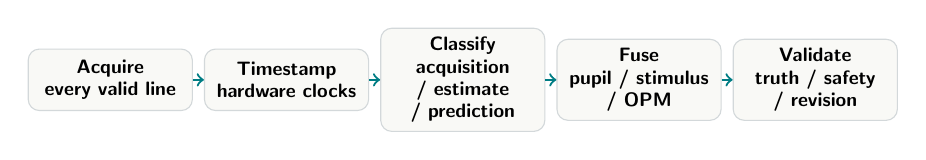
\begin{tikzpicture}[
    box/.style={draw=Light,rounded corners,text width=1.85cm,minimum height=.78cm,
                align=center,fill=OffWhite,font=\scriptsize},
    arr/.style={->,thick,Teal}
  ]
    \node[box] (a) {\bfseries Acquire\\every valid line};
    \node[box,right=.14cm of a] (t) {\bfseries Timestamp\\hardware clocks};
    \node[box,right=.14cm of t] (c) {\bfseries Classify\\acquisition / estimate / prediction};
    \node[box,right=.14cm of c] (f) {\bfseries Fuse\\pupil / stimulus / OPM};
    \node[box,right=.14cm of f] (v) {\bfseries Validate\\truth / safety / revision};
    \draw[arr] (a)--(t); \draw[arr] (t)--(c); \draw[arr] (c)--(f); \draw[arr] (f)--(v);
  \end{tikzpicture}
  \end{center}
  \vspace{0.25cm}
  \takeaway{Near-term decision: freeze line-stream, clock, calibration, safety, and multimodal
    interfaces before freezing production hardware.}
  \source{engineering evidence and strategic audit}
\end{frame}

\end{document}
